\chapter{Results and Discussion}
\label{Chapter5}

This chapter reports what was measured with the framework of Chapter~\ref{Chapter4} and discusses it. Section~\ref{sec:ch5-experiments} lists the experiments and gives the measurements of the uncompressed model. Section~\ref{sec:ch5-stage0} reports the Stage~0 profile. Sections~\ref{sec:ch5-quant}, \ref{sec:ch5-prune} and \ref{sec:ch5-kv} report the three single-stage paths, and Section~\ref{sec:ch5-search} reports the sequential path and the search. Section~\ref{sec:ch5-discussion} answers the research questions of Chapter~1 and Section~\ref{sec:ch5-limits} states the limitations of the evidence. In every table and figure a lower perplexity, a smaller size and a lower latency are better, and a higher accuracy and a higher number of tokens per second are better.

\section{Experiments and the FP16 Reference}
\label{sec:ch5-experiments}

Table~\ref{tab:ch5-experiments} lists the experiments. All of them use TinyLlama, the seed 0 and the data of Section~\ref{sec:ch4-data}. The single-stage experiments use the default Stage~0 settings, a sensitivity threshold $\tau = 0.5$ and, for quantization, a group size of 128 weights.

\begin{table}[htbp]
\centering
\small
\caption{The experiments reported in this chapter.}
\label{tab:ch5-experiments}
\renewcommand{\arraystretch}{1.2}
\begin{tabularx}{\textwidth}{>{\raggedright\arraybackslash}p{2.9cm}X>{\raggedright\arraybackslash}p{1.7cm}>{\raggedright\arraybackslash}p{2.7cm}}
\hline
\textbf{Path} & \textbf{What was run} & \textbf{GPU} & \textbf{Engines measured} \\
\hline
0 $\rightarrow$ 1 $\rightarrow$ 4 & 11 weight techniques and 12 combined techniques, as Standard and as Our method & RTX~5070~Ti & Hugging Face, llama.cpp \\
0 $\rightarrow$ 2 $\rightarrow$ 4 & 3 pruning techniques at levels of 30 to 90 percent, as Standard, as Our method and with the same-size plan (61 rows; structured pruning up to 80 percent) & A100 & Hugging Face, llama.cpp, vLLM \\
0 $\rightarrow$ 3 $\rightarrow$ 4 & 6 KV-cache techniques, as Standard and as Our method & A100 & Hugging Face \\
0 $\rightarrow$ 1 $\rightarrow$ 2 $\rightarrow$ 3 $\rightarrow$ 4 & Search runs of 30 or 40 tries; each try is one model built through Stages~1, 2 and 3 & A100 & Hugging Face, vLLM \\
\hline
\end{tabularx}
\end{table}

The RTX~5070~Ti is the GPU of the host PC. The row count includes the FP16 row. No TensorRT-LLM measurement is reported in this chapter; the measured engines are Hugging Face Transformers, llama.cpp and vLLM.

Table~\ref{tab:ch5-fp16} gives the measurements of the uncompressed FP16 model, which is the reference for everything that follows. As explained in Section~\ref{sec:ch4-export}, llama.cpp scores only the second half of each window, so its perplexity (8.12) is comparable with other llama.cpp perplexities and not with the Hugging Face and vLLM value (10.18).

\begin{table}[htbp]
\centering
\small
\caption{The uncompressed FP16 model. Perplexity is given on the validation set and on the held-out set.}
\label{tab:ch5-fp16}
\renewcommand{\arraystretch}{1.2}
\begin{tabularx}{\textwidth}{lX}
\hline
\textbf{Engine} & \textbf{Measurement} \\
\hline
Hugging Face & Perplexity 10.18 / 10.62; decode 4.32~ms per token and prefill 5.87~ms on the RTX~5070~Ti; decode 4.24~ms per token on the A100; peak GPU memory 2.41~GB \\
llama.cpp & File 2.20~GB; perplexity 8.12 / 8.56; 324 tokens per second on the RTX~5070~Ti and 421 on the A100 \\
vLLM (A100) & File 2.20~GB; perplexity 10.18 / 10.62; decode 2.54~ms per token; prefill 9.16~ms; peak GPU memory 3.77~GB \\
Accuracy & ARC-Easy 0.548, PIQA 0.745, HellaSwag 0.604, WinoGrande 0.603; mean 0.625 \\
\hline
\end{tabularx}
\end{table}

\section{Stage 0: Layer Sensitivity}
\label{sec:ch5-stage0}

Figure~\ref{fig:ch5-sensitivity} shows the raw sensitivity score of Equation~\ref{eq:ch4-score} for the 22 decoder layers. The perplexity of the unchanged model on the calibration text is 14.12. Bypassing layer~0 raises it by 1{,}176 and bypassing layer~2 by 368. Three more layers have a rise above 10: layer~7 (36.5), layer~21 (23.6) and layer~1 (11.6). For the other 17 layers the rise is between 1.4 and 5.7. The sensitivity is therefore very uneven: the largest score is about 800 times the smallest, and the five largest scores belong to the first three layers, one middle layer and the last layer. These five layers are the guarded layers, which are never pruned.

\begin{figure}[htbp]
\centering
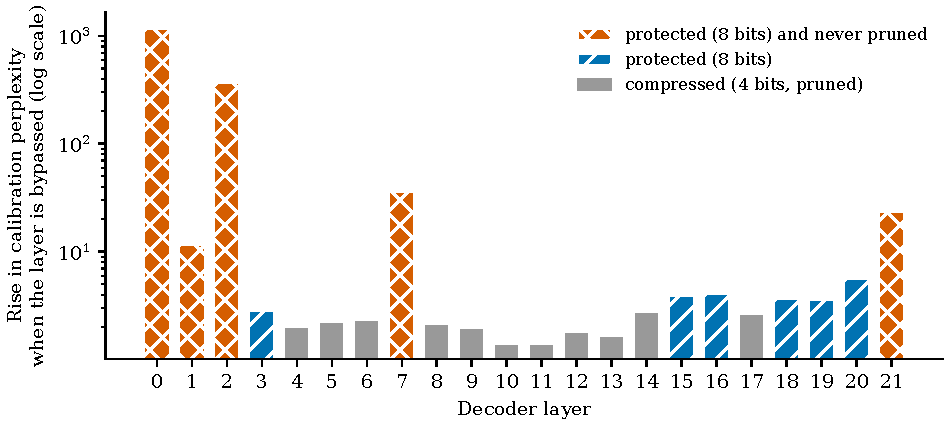
\includegraphics[width=0.95\textwidth]{Figures/ch5-sensitivity.pdf}
\caption{Stage~0 sensitivity score of each decoder layer (log scale; a higher bar is a more sensitive layer) and the weight plan at the default threshold $\tau = 0.5$.}
\label{fig:ch5-sensitivity}
\end{figure}

At the default threshold the weight plan protects 11 of the 22 layers (layers 0, 1, 2, 3, 7, 15, 16, 18, 19, 20 and 21), which keep 8 bits and are not pruned; the other 11 layers get 4 bits and the pruning ratio. The activation plan gives 8 bits to 11 layers and 4 bits to the other 11, an average of 6 bits. The KV-cache plan keeps the keys and values of every layer at 4 bits, except the values of layer~0 at 2 bits, and lets each layer keep between 10 and 100 percent of the past tokens; over the whole cache it keeps 25.9 percent of the tokens at an average of 3.82 bits.

The profile is cheap. The 23 passes over the calibration text that give the scores took 96~s on the RTX~5070~Ti and 121~s on the A100. The activation measurements took 188~s and building the KV-cache plan took 541~s on the RTX~5070~Ti. All of them are computed once and reused from the cache by every later run.

\section{Quantization (Path 0 $\rightarrow$ 1 $\rightarrow$ 4)}
\label{sec:ch5-quant}

\subsection{Weights Only}

Table~\ref{tab:ch5-quant-wo} and Figure~\ref{fig:ch5-quant} compare the eleven weight techniques on the Standard plan (4 bits in every layer) and on the Stage~0 plan (8 bits in the 11 protected layers, 4 bits in the others).

\begin{table}[htbp]
\centering
\small
\caption{Weight-only quantization, Standard (Std) against Our method (Ours), measured on the RTX~5070~Ti. Perplexity: lower is better. Tokens per second: higher is better. The llama.cpp file is 0.81~GB for every Standard row and 1.05~GB for every Our method row; the FP16 file is 2.20~GB.}
\label{tab:ch5-quant-wo}
\renewcommand{\arraystretch}{1.15}
\begin{tabularx}{\textwidth}{Xrrrrrrrr}
\hline
 & \multicolumn{2}{c}{\textbf{Hugging Face}} & \multicolumn{2}{c}{\textbf{Hugging Face}} & \multicolumn{2}{c}{\textbf{llama.cpp}} & \multicolumn{2}{c}{\textbf{llama.cpp}} \\
 & \multicolumn{2}{c}{\textbf{validation}} & \multicolumn{2}{c}{\textbf{held-out}} & \multicolumn{2}{c}{\textbf{validation}} & \multicolumn{2}{c}{\textbf{tokens/s}} \\
\textbf{Technique} & Std & Ours & Std & Ours & Std & Ours & Std & Ours \\
\hline
FP16 & \multicolumn{2}{c}{10.18} & \multicolumn{2}{c}{10.62} & \multicolumn{2}{c}{8.12} & \multicolumn{2}{c}{324} \\
\hline
@@QUANT_WO@@
\hline
\end{tabularx}
\end{table}

\begin{figure}[htbp]
\centering
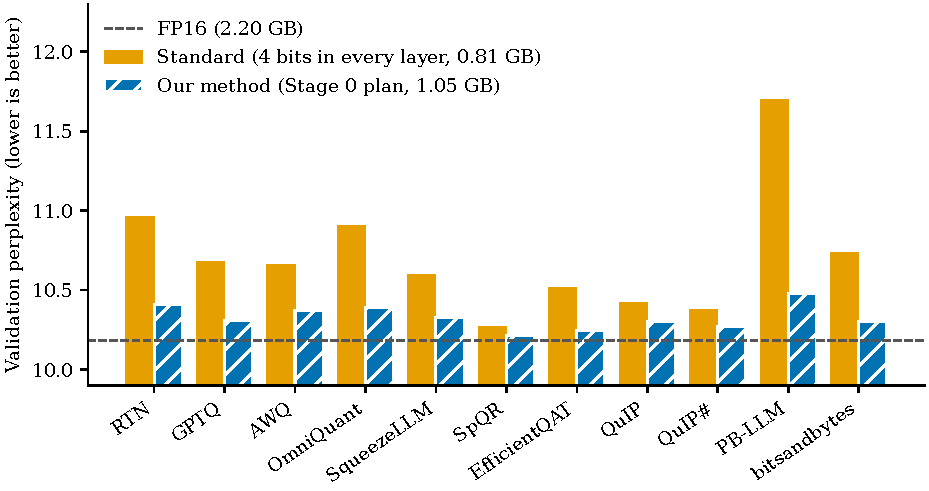
\includegraphics[width=0.95\textwidth]{Figures/ch5-quantization.pdf}
\caption{Hugging Face validation perplexity of weight-only quantization (lower is better). The dashed line is the FP16 model.}
\label{fig:ch5-quant}
\end{figure}

\textbf{What this shows.} Our method has a lower perplexity than Standard for all eleven techniques, on the validation set and on the held-out set, in Hugging Face and in llama.cpp. The gain is largest for the techniques that lose most at 4 bits: PB-LLM improves from 11.70 to 10.48 and round-to-nearest from 10.97 to 10.41. It is smallest for the technique that is already close to FP16: SpQR improves from 10.27 to 10.21. With Our method every technique is between 10.21 and 10.48, so the choice of technique matters much less than on the Standard plan, where the range is 10.27 to 11.70.

\textbf{What it costs.} The Our method file is larger, 1.05~GB against 0.81~GB, because half of the layers keep 8 bits. It is also slower in llama.cpp: 532 to 559 tokens per second against 624 to 655. Both are still well ahead of the FP16 model, which needs 2.20~GB and reaches 324 tokens per second on the same GPU. The comparison is therefore not at equal size. Our method buys back a part of the quality lost at 4 bits (for round-to-nearest, 71 percent of the gap between the 4-bit model and FP16) for 0.24~GB of extra file size and about 15 percent of the llama.cpp speed.

\textbf{What Hugging Face does not show.} The decode latency of the simulated model in Hugging Face is between 4.09 and 4.22~ms per token for every weight-only row, against 4.32~ms for FP16. The simulated model stores rounded values in 16-bit tensors, so it cannot be faster or smaller; the real gain appears only in the exported file.

\subsection{Weights and Activations}

Table~\ref{tab:ch5-quant-wa} reports the combined techniques. The Standard row uses 4-bit weights and 8-bit activations in every layer. The Our method row uses the Stage~0 quantization plan and the Stage~0 activation plan, which averages 6 bits. A second Our method row uses the joint weight and activation plan, and a second Standard row uses 8-bit weights and 8-bit activations in every layer.

\begin{table}[htbp]
\centering
\small
\caption{Weights and activations: Hugging Face validation perplexity (lower is better), measured on the RTX~5070~Ti. Each weight technique is combined with round-to-nearest activations unless stated.}
\label{tab:ch5-quant-wa}
\renewcommand{\arraystretch}{1.15}
\begin{tabularx}{\textwidth}{Xrrrr}
\hline
\textbf{Weight technique} & \textbf{Standard} & \textbf{Our method} & \textbf{Our method,} & \textbf{Standard,} \\
 & \textbf{(4-bit weights,} & \textbf{(weight plan,} & \textbf{joint plan} & \textbf{8-bit weights,} \\
 & \textbf{8-bit activations)} & \textbf{activation plan)} & & \textbf{8-bit activations} \\
\hline
@@QUANT_WA@@
\hline
\end{tabularx}
\end{table}

\textbf{What this shows.} With rounded activations the picture changes. Our method is better than Standard for four of the twelve techniques (round-to-nearest, OmniQuant, PB-LLM and round-to-nearest with SmoothQuant) and worse for the other eight; for SpQR the perplexity rises from 10.28 to 10.64. The reason is in the plans: Our method gives more bits to the weights of the protected layers, but its activation plan gives 4 bits to half of the layers, where the Standard plan gives 8 bits to all of them. For the techniques whose 4-bit weights are already good, the loss from the 4-bit activations is larger than the gain from the 8-bit weights. The joint plan gives almost the same result as the separate plans. With 8 bits everywhere, every technique is within 0.04 of the FP16 perplexity, at a llama.cpp file of 1.29~GB.

\textbf{What it means.} A per-layer plan helps where the uniform setting is short of bits (4-bit weights) and does not help where the uniform setting is already generous (8-bit activations) and the plan spends fewer bits than it.

\section{Pruning (Path 0 $\rightarrow$ 2 $\rightarrow$ 4)}
\label{sec:ch5-prune}

Figure~\ref{fig:ch5-prune} and Table~\ref{tab:ch5-prune} report the three pruning techniques. At a pruning level of 30 percent the Standard plan removes 30 percent of every decoder layer, which is 26 percent of all parameters of the model. The Our method plan removes 30 percent of the 11 compressed layers only, which is 13 percent of all parameters. The same-size plan removes the same total as the Standard plan but places it by sensitivity: nothing in the five guarded layers and up to 61 percent in the most robust layer.

\begin{figure}[htbp]
\centering
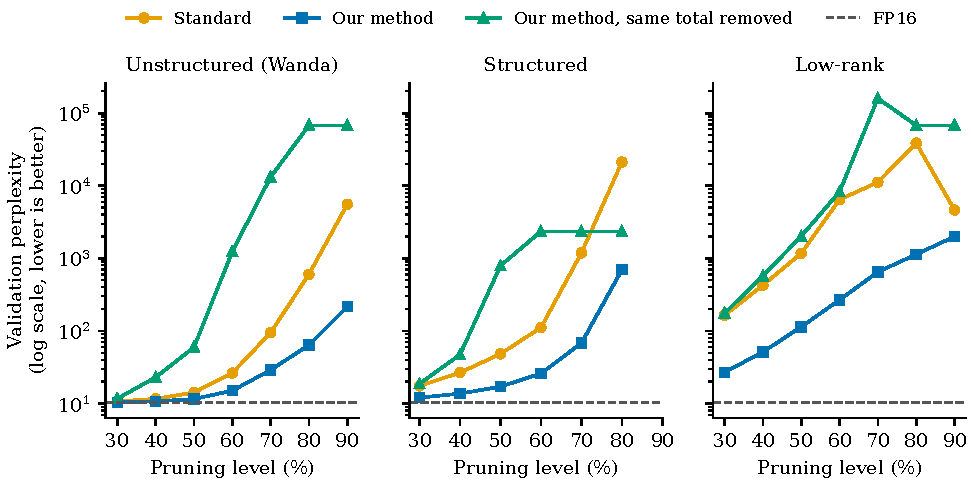
\includegraphics[width=\textwidth]{Figures/ch5-pruning.pdf}
\caption{Hugging Face validation perplexity after pruning, against the pruning level (log scale; lower is better). The dashed line is the FP16 model.}
\label{fig:ch5-prune}
\end{figure}

\begin{table}[htbp]
\centering
\small
\caption{Hugging Face validation perplexity after pruning (lower is better), measured on the A100. FP16: 10.18.}
\label{tab:ch5-prune}
\renewcommand{\arraystretch}{1.1}
\begin{tabularx}{0.9\textwidth}{Xrrrr}
\hline
\textbf{Technique} & \textbf{Level (\%)} & \textbf{Standard} & \textbf{Our method} & \textbf{Our method,} \\
 & & & & \textbf{same total removed} \\
\hline
@@PRUNE@@
\hline
\end{tabularx}
\end{table}

\textbf{What this shows.} Our method has a lower perplexity than Standard at every level for all three techniques (20 of 20 comparisons). With unstructured pruning at 50 percent the perplexity is 11.51 against 14.12, and at 70 percent 28.85 against 94.55. As in quantization, the comparison is not at equal size, because Our method removes about half as many weights. The same-size plan gives the comparison at equal size, and it is worse than Standard in 19 of the 20 comparisons: at 30 percent unstructured pruning 11.60 against 10.66. Moving the pruning away from the sensitive layers and concentrating it on the robust ones does more damage than spreading it evenly. Of the three techniques, unstructured pruning loses least, structured pruning is clearly worse (17.47 at 30 percent on the Standard plan) and the low-rank factorisation is the worst (163).

\textbf{What the engines show.} Pruned weights are stored as zeros, and the engines confirm that this brings nothing: the llama.cpp file and the vLLM file are 2.20~GB in all 61 rows, the vLLM decode latency is between 2.51 and 2.55~ms per token in all rows (FP16: 2.54), and llama.cpp runs at 412 to 426 tokens per second (FP16: 421). Because the weights of a pruned model are exported at 16 bits without re-rounding, the vLLM perplexity agrees with the Hugging Face perplexity to within 0.05 percent in every row.

\section{KV-cache Compression (Path 0 $\rightarrow$ 3 $\rightarrow$ 4)}
\label{sec:ch5-kv}

Table~\ref{tab:ch5-kv} reports the six KV-cache techniques. The cache memory is the memory that the setting needs for a context of 2{,}048 tokens and a batch of one; the FP16 cache needs 46.1~MB. The Standard rounding techniques use 4 bits for every key and value and keep every token (13.0~MB). The Standard eviction techniques keep 20 percent of the tokens at 16 bits (9.2~MB). Our method applies the Stage~0 KV-cache plan, which both rounds and evicts, and needs 3.2~MB.

\begin{table}[htbp]
\centering
\small
\caption{KV-cache compression, measured in Hugging Face on the A100. Perplexity on the validation set and on the held-out set (lower is better); cache memory for 2{,}048 tokens (smaller is better). FP16: 10.18 / 10.62 with 46.1~MB.}
\label{tab:ch5-kv}
\renewcommand{\arraystretch}{1.15}
\begin{tabularx}{\textwidth}{Xrrrrrr}
\hline
 & \multicolumn{3}{c}{\textbf{Standard}} & \multicolumn{3}{c}{\textbf{Our method}} \\
\textbf{Technique} & Val. & Held-out & MB & Val. & Held-out & MB \\
\hline
@@KV@@
\hline
\end{tabularx}
\end{table}

\textbf{What this shows.} For five of the six techniques the Our method row has a higher perplexity than the Standard row, and it uses a cache that is 4.0 times smaller than the Standard rounding cache and 2.9 times smaller than the Standard eviction cache. The exception is InfiniGen, where Our method is better on both counts: 10.38 against 11.00 with about a third of the memory. The three Standard rounding techniques stay close to FP16 (10.25 to 10.33), which shows that 4-bit keys and values cost little on this model; most of the loss in the Our method rows comes from the tokens that the plan evicts. The Our method rows of round-to-nearest KV and H2O are equal because under the plan the two techniques apply the same rounding and keep the same tokens.

\textbf{What it means.} The KV-cache plan trades quality for memory rather than improving both. Whether it is a good trade depends on the technique that carries it out: with InfiniGen the plan gives the lowest perplexity of all KV-cache rows at the smallest cache. The KV-cache techniques exist only in the Hugging Face model, so these results describe quality and cache size, not speed.

\section{Sequential Path and Search}
\label{sec:ch5-search}

In the sequential path one model is quantized, then pruned, then given a KV-cache technique, and the search of Section~\ref{sec:ch4-search} chooses the three techniques and the plan settings. All searches in this section use the Bayesian optimiser and the search ranges of Table~\ref{tab:ch4-space} unless stated. Following Section~\ref{sec:ch1-scope}, the searches are reported as outcomes.

\subsection{Searches under the Two Limits}

Table~\ref{tab:ch5-searches} lists the searches that were run under the requirement of Section~\ref{sec:ch4-requirement}: a validation perplexity of at most 11.5 and a vLLM decode latency of at most 2.5~ms per token.

\begin{table}[htbp]
\centering
\footnotesize
\caption{Searches under the limits of perplexity at most 11.5 and vLLM decode latency at most 2.5~ms per token. HF: Hugging Face. The FP16 model has a perplexity of 10.18 and a vLLM decode latency of 2.54~ms per token.}
\label{tab:ch5-searches}
\renewcommand{\arraystretch}{1.2}
\begin{tabularx}{\textwidth}{>{\raggedright\arraybackslash}p{4.3cm}lrr>{\raggedright\arraybackslash}X}
\hline
\textbf{Search (objectives in order)} & \textbf{Perplexity} & \textbf{Tries} & \textbf{Within} & \textbf{Outcome} \\
 & \textbf{judged in} & & \textbf{both limits} & \\
\hline
Lowest perplexity, then lowest latency, then smallest size & HF & 30 & 2 & Final model: 0.84~GB, 1.98~ms (Table~\ref{tab:ch5-finals}) \\
The same, with weight-only quantization only & HF & 30 & 17 & Final model: 0.90~GB, 2.00~ms (Table~\ref{tab:ch5-finals}) \\
The same as the first, with a perplexity limit of 11.0 & HF & 30 & 0 & Closest try: perplexity 11.50 at 2.0~ms \\
The same as the first, with a latency limit of 2.0~ms & HF & 30 & 1 & In effect the final model of the first search (same technique and calibration, perplexity 11.50) \\
The same as the first, with structured pruning only & HF & 30 & 0 & Closest try: perplexity 11.52 at 1.99~ms, with nothing pruned \\
Smallest size, then lowest perplexity, then lowest latency & HF & 30 & 0 & Fast tries at perplexity 11.75 or higher; the tries below 11.5 decode in about 42~ms \\
The same as the first, repeated with 40 tries & HF & 40 & 0 & Closest fast try: perplexity 11.75 at 2.14~ms \\
Lowest perplexity, then smallest size & vLLM & 40 & 0 & Figure~\ref{fig:ch5-tries}, left \\
Fastest, then smallest size & vLLM & 40 & 0 & Figure~\ref{fig:ch5-tries}, right \\
\hline
\end{tabularx}
\end{table}

Two searches gave a final model. Their settings and measurements are in Table~\ref{tab:ch5-finals}, next to the FP16 model and to two models from earlier searches that are described in Section~\ref{sec:ch5-smallest}.

\begin{table}[htbp]
\centering
\footnotesize
\caption{The final models, measured in vLLM on the A100, and their accuracy. Perplexity is given on the validation set and on the held-out set. Lower is better for size, perplexity, latency and memory; higher is better for accuracy.}
\label{tab:ch5-finals}
\renewcommand{\arraystretch}{1.2}
\begin{tabularx}{\textwidth}{>{\raggedright\arraybackslash}p{2.25cm}>{\raggedright\arraybackslash}p{1.15cm}>{\raggedright\arraybackslash}X>{\raggedright\arraybackslash}X>{\raggedright\arraybackslash}X>{\raggedright\arraybackslash}X}
\hline
 & \textbf{FP16} & \textbf{Lowest-perplexity search} & \textbf{Weight-only search} & \textbf{Smallest-size search} & \textbf{Smallest-size search, narrower ranges} \\
\hline
Quantization & none & OmniQuant, weights only; threshold 0.857; per channel; C4, 32 windows & Round-to-nearest, weights only; threshold 0.800; group 64; C4, 128 windows & GPTQ with round-to-nearest activations; threshold 0.759; group 128; WikiText-2, 64 windows & SqueezeLLM with SmoothQuant (strength 0.638); threshold 0.876; group 32; Pile, 128 windows \\
Pruning & none & Unstructured, ratio 0.082 & Unstructured, ratio 0 (nothing removed) & Unstructured, ratio 0 (nothing removed) & Unstructured, ratio 0.262 \\
KV cache & none & InfiniGen & SnapKV & InfiniGen & InfiniGen \\
\hline
vLLM file (GB) & 2.200 & 0.838 & 0.898 & 0.894 & 0.873 \\
HF perplexity & 10.18 / 10.62 & 11.50 / 11.91 & 11.12 / 11.52 & 11.23 / 11.62 & 11.44 / 11.87 \\
vLLM perplexity & 10.18 / 10.62 & 13.00 / 13.41 & 11.10 / 11.54 & 12.09 / 12.52 & 11.46 / 11.89 \\
vLLM decode (ms per token) & 2.54 & 1.98 & 2.00 & 34.42 & 42.45 \\
vLLM peak memory (GB) & 3.77 & 2.40 & 2.45 & 2.46 & 2.44 \\
\hline
ARC-Easy & 0.548 & 0.443 & 0.325 & 0.402 & 0.415 \\
PIQA & 0.745 & 0.691 & 0.630 & 0.676 & 0.676 \\
HellaSwag & 0.604 & 0.566 & 0.516 & 0.551 & 0.555 \\
WinoGrande & 0.603 & 0.523 & 0.510 & 0.521 & 0.509 \\
Mean accuracy & 0.625 & 0.556 & 0.495 & 0.538 & 0.539 \\
\hline
\end{tabularx}
\end{table}

\textbf{The lowest-perplexity search.} Two of its 30 tries were within both limits. The final model uses OmniQuant on the weights only (sensitivity threshold 0.857, per-channel groups, calibrated on 32 windows of C4), unstructured pruning with a ratio of 0.082 and InfiniGen for the KV cache. Its vLLM file is 0.838~GB, 62 percent smaller than the FP16 file, and it decodes in 1.98~ms per token, 22 percent faster than FP16. Its perplexity is 11.50 in Hugging Face but 13.00 in vLLM, and its mean accuracy is 0.556 against 0.625 for FP16, a relative drop of 11.1 percent.

\textbf{The weight-only search.} When Stage~1 was restricted to weight-only techniques, 17 of the 30 tries were within both limits. The final model uses round-to-nearest on the weights only (threshold 0.800, which gives 8 bits to the five layers 0, 1, 2, 7 and 21; groups of 64 weights; calibrated on 128 windows of C4), unstructured pruning with a ratio of 0, so that nothing is removed, and SnapKV for the KV cache. Its vLLM file is 0.898~GB (59 percent smaller than FP16) and it decodes in 2.00~ms per token (21 percent faster). Its perplexity is almost the same in both engines, 11.12 in Hugging Face and 11.10 in vLLM, so this model is within both limits also when the perplexity is judged in vLLM. Its mean accuracy is 0.495, a relative drop of 20.8 percent, the largest of the final models, although its perplexity is the lowest of them.

\textbf{Tighter limits and other variants.} Lowering the perplexity limit to 11.0 left no try within the limits, and lowering the latency limit to 2.0~ms left one, which is in effect the final model of the first search. With structured pruning as the only Stage~2 technique, the closest try pruned nothing and reached 11.52. With size as the first objective, no try was within the limits. A repeat of the first search with 40 tries, made with a later version of the code, also had no try within both limits; its closest fast try had a perplexity of 11.75.

\textbf{Perplexity judged in vLLM.} Because the perplexity of an exported model can differ from its Hugging Face perplexity, the last two searches checked the perplexity limit on the model as loaded in vLLM. Figure~\ref{fig:ch5-tries} shows all 40 tries of each. The tries fall into two groups. The 30 weight-only tries, all of which used OmniQuant, decode in 1.97 to 2.14~ms per token, faster than FP16, with a vLLM file of 0.82 to 0.86~GB, but their vLLM perplexity is 12.97 or higher. The 10 tries with rounded activations decode in 33 to 43~ms per token; one of them reaches a vLLM perplexity of 10.98. No try is within both limits. Round-to-nearest as a weight-only technique, which gave the final model of the weight-only search, was not proposed in these tries.

\begin{figure}[htbp]
\centering
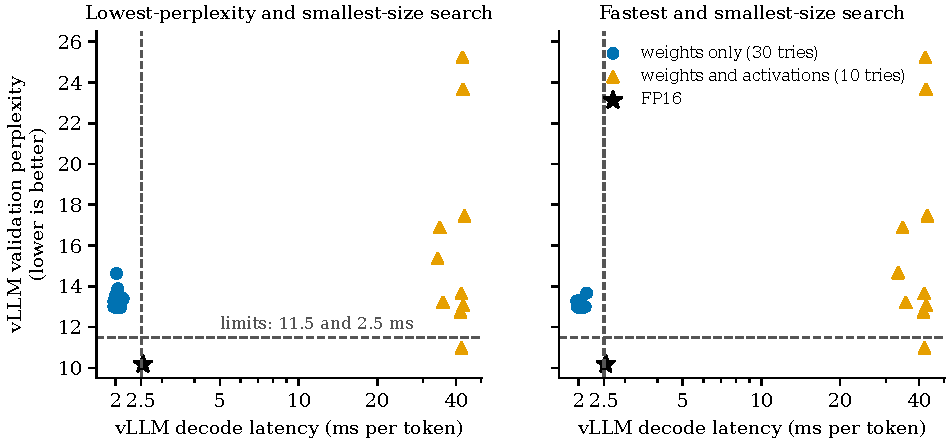
\includegraphics[width=\textwidth]{Figures/ch5-search-tries.pdf}
\caption{All 40 tries of the two searches that judge perplexity in vLLM. Lower and further left is better. The dashed lines are the two limits; a try within both limits would lie in the lower left corner.}
\label{fig:ch5-tries}
\end{figure}

\subsection{Searches for the Smallest Model}
\label{sec:ch5-smallest}

Before the latency limit was introduced, searches were run with the perplexity limit only (Hugging Face perplexity at most 11.5) and with the predicted weight memory as the first objective. The first of the two final models in Table~\ref{tab:ch5-finals} comes from a search over the full ranges of Table~\ref{tab:ch4-space} and uses GPTQ with round-to-nearest activations; the second comes from a search over the narrower ranges, in which a layer could also be given 3 bits, and uses SqueezeLLM with SmoothQuant; no layer of this final model has 3 bits. Both are small, 0.894 and 0.873~GB in vLLM, and both are within the perplexity limit in Hugging Face. Both keep the activations at low bit widths, and in vLLM they decode in 34.4 and 42.5~ms per token, 13.5 and 16.7 times slower than FP16. A small file is therefore not a fast model, and this is what led to the latency limit.

These two searches were also run with successive halving on the same search space and seed, which gives the comparison of Table~\ref{tab:ch5-optimisers}. In both, the Bayesian optimiser found a smaller model within the limit, with fewer models built and in less time.

\begin{table}[htbp]
\centering
\small
\caption{Bayesian optimisation against successive halving in the two searches for the smallest model with a Hugging Face perplexity of at most 11.5.}
\label{tab:ch5-optimisers}
\renewcommand{\arraystretch}{1.15}
\begin{tabularx}{\textwidth}{llrrr>{\raggedright\arraybackslash}X}
\hline
\textbf{Search} & \textbf{Optimiser} & \textbf{Models} & \textbf{Build time} & \textbf{Within} & \textbf{Smallest model within the limit} \\
 & & \textbf{built} & & \textbf{the limit} & \textbf{(predicted size, perplexity)} \\
\hline
First & Bayesian & 30 & 245 min & 4 & 0.924~GB at 11.39 \\
 & Successive halving & 129 & 495 min & 10 & 0.939~GB at 11.44 \\
Second & Bayesian & 30 & about 190 min & 8 & 0.868~GB at 11.42 \\
 & Successive halving & 130 & about 500 min & 0 & none (closest: 0.916~GB at 11.66) \\
\hline
\end{tabularx}
\end{table}

\section{Discussion}
\label{sec:ch5-discussion}

This section answers the five research questions of Chapter~1 with the evidence above.

\textbf{RQ1: how uneven is the sensitivity, and does the score predict the damage?} The sensitivity is very uneven: five of the 22 layers have a score above 10 and two of them above 300, while the other 17 are between 1.4 and 5.7 (Figure~\ref{fig:ch5-sensitivity}). The score is a useful guide for protection. Giving the protected layers 8 bits lowered the perplexity of all eleven weight techniques, and leaving them unpruned lowered the perplexity of all three pruning techniques at every level. The score is not a good guide for how much more to compress the other layers: the same-size pruning plan, which moves the pruning from the sensitive layers onto the robust ones, was worse than uniform pruning in 19 of 20 comparisons. A layer that can be bypassed with little damage cannot, on this evidence, absorb a much larger share of the pruning.

\textbf{RQ2: does the per-layer plan improve the trade-off?} For weight-only quantization it improves quality at a cost in size and speed: every technique moves closer to FP16, the file grows from 0.81 to 1.05~GB and llama.cpp slows from about 650 to about 550 tokens per second. This is a different point on the trade-off, between the uniform 4-bit and the uniform 8-bit model, and not a gain at equal size. For rounded activations the plan was worse than the uniform 8-bit setting for eight of twelve techniques, because it spends fewer activation bits. For the KV cache the plan gives a cache 3 to 4 times smaller at a higher perplexity for five of six techniques, and is better on both counts with InfiniGen. The plan is most useful with simple techniques: it brings round-to-nearest (10.41) close to what the best technique reaches on the uniform plan (SpQR, 10.27).

\textbf{RQ3: quantization only, pruning only, or both?} In the engines studied here quantization is the only stage that reduces the file size and the latency. Pruning costs perplexity and returns nothing in size or speed, because the removed weights are stored as zeros (Section~\ref{sec:ch5-prune}). The searches agree: the final models within both limits prune nothing or very little (ratios of 0 and 0.082), and with structured pruning only, the best try pruned nothing. On this evidence a quantization-only pipeline is preferable for these engines, and pruning becomes worth its quality cost only where the engine or the hardware can exploit the zeros. A KV-cache technique reduces cache memory and does not change the exported model.

\textbf{RQ4: how do the simulated results carry over to the engines?} Three differences were observed. First, quality carries over exactly when the weights are exported without re-rounding (the pruned models agree to within 0.05 percent between Hugging Face and vLLM), but not when the export re-rounds them: the OmniQuant final model moves from 11.50 to 13.00 and the GPTQ final model from 11.23 to 12.09, while the round-to-nearest final model stays at 11.1 and one try with rounded activations is better in vLLM (10.98) than in Hugging Face (12.06). Second, speed cannot be read from the simulation: in Hugging Face the weight-only models decode in about the same time as FP16, while in the engines they are faster (about 2.0~ms against 2.54~ms in vLLM, and 1.7 to 2.0 times the FP16 tokens per second in llama.cpp). Third, the kind of quantization decides the kernel: weight-only models are faster than FP16 in vLLM, and models with rounded activations are 13 to 17 times slower. A model should therefore be selected on measurements made in the engine that will serve it.

\textbf{RQ5: can the search find configurations that meet a deployment requirement?} In part. With the perplexity judged in Hugging Face, two searches found models within both limits, and both final models are about 60 percent smaller and about 20 percent faster than FP16 in vLLM. The final model of the weight-only search is within both limits in vLLM as well. With the perplexity judged in vLLM, 40 tries of each of two searches found fast models and low-perplexity models but none that is both. The search also showed what the requirement leaves out: perplexity did not rank the final models by accuracy, since the model with the lowest perplexity lost the most accuracy (20.8 percent) and every final model lost at least 11 percent. A requirement that is meant to protect task accuracy needs an accuracy measurement among its limits.

\textbf{Relation to the five gaps.} The single-stage experiments compare 4-bit, plan-based and 8-bit precision under identical conditions (gap one). The pruning and search results give a rule for the pipeline in these engines: quantize, and prune only if the engine can use it (gaps two and three). Every result is reported per engine, and the differences between the simulation and the engines are measured (gap four). The plan and the search choose the bit widths, the pruning ratio and the techniques from a stated requirement (gap five).

\section{Limitations of the Evidence}
\label{sec:ch5-limits}

The results hold for one model, TinyLlama, and one seed; the variation between seeds was not measured, so small differences between rows should not be over-read. Most techniques are simplified re-implementations (Section~\ref{sec:ch1-scope}), and their numbers are not the numbers of the original methods. Standard and Our method differ in size in the quantization and pruning experiments; only the same-size pruning plan is a comparison at equal size, and no equal-size comparison was made for quantization. The cache memory of the KV-cache techniques is computed from the plan and not measured in an engine, and the KV-cache techniques could not be exported. Latency was measured at a batch of one with a prompt of 128 tokens and 64 generated tokens, on two GPUs. Accuracy was measured for the final models only. No TensorRT-LLM measurement is reported. In the searches, the number of tries is small compared with the size of the search space, and a search that found no try within the limits does not show that no such configuration exists.
